\chapter{Postulats et évolution temporelle}
\label{chap:postu}
\minitoc

\bigskip


Nous sommes maintenant suffisamment éclairés sur la \emph{magie} du monde
quantique pour procéder à une généralisation des résultats et principes établis
jusqu'alors à travers les postulats de base de la théorie quantique
(\textbf{section \ref{sec:PostMQ}}). Ces postulats fixent cadre conceptuel
général de la dite théorie. A la \textbf{section \ref{sec:EvolTempo}}, on
s'intéresse à l'évolution temporelle des états quantiques en mettant l'accent
sur les états stationnaires ou états propres de l'énergie. Le chapitre s'achève
avec la \textbf{section \ref{sec:ESpin12}} avec les oscillations de Rabi,
exemples de manipulations des qubits.

\section{Postulats de la théorie quantique}
\label{sec:PostMQ}

\subsection{Postulat 1: Espace des états}

\colorbox[gray]{0.8}{
\parbox[c]{0.9\textwidth}{
\emph{L'état physique d'un système est \textbf{entièrement ou complètement}
défini, à chaque instant, par un élément $\ket{\psi}$ d'un espace de Hilbert
$\mathcal{H}$ approprié.}
}}
\medskip

Toute superposition linéaire d'états
\begin{equation}
\ket{\psi}={\textstyle\sum\limits_n}\ket{\varphi_n}
\langle\varphi_n\ket{\psi} ={\textstyle\sum\limits_n}
\alpha_n\ket{\varphi_n},
\end{equation}
est un élément de $\mathcal{H}$, avec $\alpha_n\in\mathbb{C}$,
$\ket{\varphi_n}\in\mathcal{H}$. Les $\ket{\varphi_n}$ sont donc également
des vecteurs d'état et la base $\{\ket{\varphi_n}\}$ est orthonormée. Ce sont
les amplitudes de projections ou de transition $\alpha_n=\langle
\varphi_n\ket{\psi}$ de l'état $\ket{\psi}$ sur l'ensemble des états
$\ket{\varphi_n} $ du système qui caractérisent l'état du système. Autrement,
$\ket{\psi}$ \emph{\textbf{est l'être mathématique qui décrit la réalité
physique d'un état quantique individuel}}\footnote{On peut aussi dire que c'est
l'être mathématique qui décrit l'information disponible sur un système
quantique.}.

Dans l'expérience de Stern et Gerlach de la \textbf{section \ref{sec:ExpSG}},
$\ket{\psi}=\alpha_{+}\ket{+}+\alpha_{-}\ket{-}$, $\ket{+}$ et $\ket{-}$ étant
les différents états physiques (de spin) des atomes d'argent qui forme le
système quantique.

\subsection{Postulat 2: Amplitudes de probabilité et probabilités}

\colorbox[gray]{0.8}{
\parbox[c]{0.9\textwidth}{
\emph{Si $\ket{\psi}$ et $\ket{\varphi_n} $ représente les états physiques
d'un système quantique, la probabilité $\mathcal{P}(\varphi_n \leftarrow\psi)$
pour l'état $\ket{\psi}$ de passer le test $\ket{\varphi_n}$ est
(\ref{eq:Postu4}), avec $\langle\varphi_n\ket{\psi}$ est l'amplitude de
probabilité ou de transition pour que le système qui était dans l'état
$\ket{\psi}$ se trouve dans l'état $\ket{\varphi_n}$.}
}}
\medskip

Dans l'expérience de Stern et Gerlach, l'amplitude de probabilité de trouver
$\ket{\psi}$ dans l'état $\ket{+}$ est $\alpha_{+}=\langle+\ket{\psi}$,
et la probabilité pour l'état $\ket{\psi}$ de passer donc le test $\ket{+}$ est
$\mathcal{P}(+)  =|\langle+\ket{\psi}|^{2}=|\alpha_{+}|^{2}$.

\subsection{Postulat 3: Grandeurs physiques et opérateurs}

\colorbox[gray]{0.8}{
\parbox[c]{0.9\textwidth}{
\emph{A toute grandeur physique mesurable $\mathcal{A}$ (position, vitesse,
polarisation,etc,) est associé un \textbf{opérateur linéaire hermitien} $A$
agissant dans $\mathcal{H}$: $A$ est le représentant mathématique de cette
grandeur $\mathcal{A}$.}
}}
\medskip

On note que contrairement à la théorie classique, la théorie quantique décrit
de façon fondamentalement différente l'état physique d'un système et les
grandeurs physiques associées. Un état est représenté par un vecteur d'état
normé, une grandeur physique par un opérateur hermitien.

\subsection{Postulat 4: Principe de quantification et de décomposition
spectrale}

\medskip
\colorbox[gray]{0.8}{
\parbox[c]{0.9\textwidth}{
\emph{La mesure d'une grandeur physique $\mathcal{A}$ ne peut donner comme
résultat qu'une des valeurs propres de l'opérateur hermitien $A$
correspondante.}

\emph{Si $\{\ket{\varphi_n}\}$ est la base des \textbf{vecteurs propres} de
$A$,i.e.,}%
\begin{equation}
A\ket{\varphi_n} =a_n\ket{\varphi_n},
\end{equation}
\emph{alors on peut écrire $A$ sous la décomposition spectrale}%
\begin{equation}
A=\sum_n\ket{\varphi_n} a_n\bra{\varphi_n},
\end{equation}
\emph{avec $a_n$ \textbf{une valeur propre} de $A$ ou valeur résultant d'une
mesure idéale faite sur $\mathcal{A}$.}
}}\medskip

\medskip
\colorbox[gray]{0.8}{
\parbox[c]{0.9\textwidth}{
\emph{La probabilité $\mathcal{P}(a_n)$ d'obtenir comme
résultat la valeur propre $a_n$ de l'opérateur hermitien $A$ est}%
\begin{equation}
\mathcal{P}(a_n)=|\langle\varphi_n\ket{\psi}|^{2}=\langle\psi\ket{\varphi_{n
}} \langle\varphi_n\ket{\psi}=|P_n\ket{\psi}|^{2},
\label{eq:Postu4}%
\end{equation}
\emph{où $P_n=\ket{\varphi_n}\bra{\varphi_n}$ est l'opérateur projection
sur la base orthonormée $\{\ket{\varphi_n}\}$.}
}}
\medskip

Ce principe signifie l'ensemble de ces vecteurs propres d'un opérateur hermitien
forme une base complète de l'espace de Hilbert. La description d'un état en
terme d'une grandeur physique $\mathcal{A}$ quantifiée, prenant $N$ valeurs
distinctes $a_n$, repose sur la connaissance de $N$ nombres, avec lesquels on
peut calculer la probabilité d'obtenir la valeur $a_n$. L'ensemble des $a_n$
forme le \textbf{spectre} de $\mathcal{A}$.

Dans l'expérience de Stern et Gerlach, l'opérateur $S$ associé à la grandeur
physique spin $\mathcal{S}$ peut s'écrire%
\begin{equation}
S=\ket{+}\left(+\frac{\hbar}{2}\right)\bra{+}+\ket{-}\left(-\frac{\hbar}{2}
\right)\bra{-}.
\end{equation}
Les vecteurs propres $\ket{+}$ et $\ket{-}$, associés respectivement au valeurs
propres $+\frac{\hbar}{2}$ et $-\frac{\hbar}{2}$ forme une base complète de
l'espace de Hilbert et les $\{+\frac{\hbar}{2},-\frac{\hbar}{2}\}$ forme le
spectre de $S$.

\begin{remark}
\begin{enumerate}
\item Les vecteurs $\ket{\varphi_n} $ et $\ket{\varphi_n^{\prime}}
=e^{i\delta}\ket{\varphi_n}$ représente le même état physique, puisque ce ne
sont que les probabilités d'amplitude qui peuvent être mesurées:%
\begin{equation}
\left\vert \langle\varphi_n^{\prime}\ket{\psi}\right\vert
^{2}=\left\vert \langle\varphi_n\ket{\psi}\right\vert
^{2},~\forall\ket{\psi}\in\mathcal{H}.
\end{equation}
Autrement, il n'est pas possible de distinguer deux états qui diffèrent
seulement par un facteur de phase global $e^{i\delta}$.

\item Cependant, l'état physique $\lambda\ket{\varphi_1}+\mu\ket{\varphi_2}$
est différent de l'état$\lambda\ket{\varphi_1}+\mu\ket{\varphi_2^{\prime}}$.
\end{enumerate}
\end{remark}

\subsection{Postulat 5: Principe de réduction du paquet d'onde}

\colorbox[gray]{0.8}{
\parbox[c]{0.9\textwidth}{
\emph{Si la mesure d'une grandeur physique $\mathcal{A}$ sur le système dans
l'état $\ket{\psi}$ donne le résultat $a_n$, l'état du système immédiatement
après la mesure est}
\begin{equation}
\ket{\varphi_n} =\frac{P_n\ket{\psi}}{\|P_n\ket{\psi}\|}=\frac
{P_n\ket{\psi}}{\sqrt{\bra{\psi}P_n\ket{\psi}}},
\label{eq:PrReduc}
\end{equation}
\emph{la projection normée de $\ket{\psi}$ sur le sous-espace propre associé à
$a_n$. \textbf{Donc la mesure est une projection orthogonale}.}
}}
\medskip

Ce postulat, qui suppose qu'on est dans un cas de mesure QND, est l'énoncé
quantitatif de l'affirmation "\textbf{la mesure perturbe le système}". Si on
effectue une mesure sur le système qui est alors dans l'état propre
$\ket{\varphi_n} $, on trouvera de façon certaine, i.e., avec une probabilité
unité, la valeur propre $a_n$. Ce principe sous-entend que l'appareil de
mesure agit comme un objet classique et ne se préoccupe pas des détails du
processus de la mesure (\emph{point de vue de Copenhagen}).

Dans le cas du spin, si le système $\ket{\psi}$ passe avec succès le test
$\ket{+}$,
\begin{equation}
\frac{P_{+}\ket{\psi}}{\|P_{+}\ket{\psi}\|}=\frac{\ket{+}\langle+\ket{\psi}}
{\sqrt{\langle\psi\ket{+}\langle +\ket{\psi}}}=\ket{+},
\end{equation}
une mesure du spin immédiatement après donnera de façon certaine $+\frac
{\hbar}{2}$: $S\ket{+}=+\frac{\hbar}{2}\ket{+}$.

Soulignons que si $A$ et $B$ commutent, la mesure de $B$ ne fait pas perdre
les informations préalables fournies par une mesure de $A$ (et
réciproquement), mais au contraire les complète; de plus, l'ordre dans lequel
on mesure les deux opérateurs $A$ et $B$ est sans importance. Pour que l'état
du système après la mesure soit déterminé, dans tous les cas, uniquement pour
le résultat obtenu, il faut que cette mesure porte sur un ECOC.

Ajoutons que \emph{si la valeur d'une grandeur physique peut être prédite avec
certitude sans perturber en rien le système, alors il existe une réalité
physique attachée à cette grandeur: }c'est la\textbf{ réalité }EPR
(Einstein-Podolsky-Rosen).


\begin{exercise}
 A system is in the state
\begin{equation}
 \ket{\psi}=\frac{1}{\sqrt{19}}(2\ket{u_1}+2\ket{u_2}+\ket{u_3}+2\ket{u_4}+
\sqrt{6}\ket{u_5})
\end{equation}
where $\{\ket{u_i},\ i=1-5\}$, are a complete and orthonormal set of vectors.
Each $\ket{u_i}$ is an eigenstate of the system’s Hamiltonian corresponding to
the possible measurement result $H\ket{u_i}=i\varepsilon\ket{u_i}$.
\begin{enumerate}
 \item Describe the set of projection operators corresponding to the
possible measurement results.
\item Determine the probability of obtaining each measurement result. What
is the state of the system after measurement if we measure the energy to be
$3\varepsilon$?
\item What is the average energy of the system?
\end{enumerate}
\end{exercise}

\begin{footnotesize}\begin{solution}
\begin{enumerate}
 \item The possible measurement results are $\varepsilon, 2\varepsilon,
3\varepsilon, 4\varepsilon$ and $5\varepsilon$. These measurement results
correspond to the basis states $\ket{u_1},\ket{u_2},\ket{u_3}),\ket{u_4}$, and
$\ket{u_5}$ respectively. Hence the projection operators corresponding to each
measurement result are
\begin{equation}
 P_1=\ket{u_1}\bra{u_1},\; P_2=\ket{u_2}\bra{u_2},\; P_2=\ket{u_3}\bra{u_3},\;
P_4=\ket{u_4}\bra{u_4},\; P_5=\ket{u_5}\bra{u_5}.
\end{equation}
Since the $\ket{u_i}$'s are a set of orthnormal basis vectors, the completeness
relation is satified and
\begin{equation}
\sum_{i}P_i = \mathbb{I}.
\end{equation}
\item We can calculate the probability of obtaining each measurement result
using the \emph{Born rule}. First we need to check and see if the state
is normalized. This is done by calculating $\sum_{i=1}^{5}|c_i|^{2}$ and and
seeing if the result is $1$. We have
\begin{equation}
\begin{split}
 \sum_{i=1}^{5}|c_i|^{2} & =\frac{1}{19}(|2|^2 +|2|^2 +|1|^2 +|2|^2 +|\sqrt{6}|
^2)\\
  & = \frac{1}{19}(4+4+1+4+6)=1.
\end{split}
\end{equation}
The state is normalized, so we can proceed. Before doing so, recall that the
fact that the basis states are orthonormal means that $\bra{u_i}\ket{u_j}
=\delta_{ij}$. So, in the first case, applying the Born rule we have
\begin{subequations}
\begin{align}
 \mathcal{\varepsilon}&=|\bra{u_1}\psi\rangle|^{2}=\langle\psi\ket{u_1}
\bra{u_1}\psi\rangle=\frac{|2|^2}{19}=\frac{4}{19},\\
 \mathcal{\varepsilon}& =|\bra{u_2}\psi\rangle|^{2}=\langle\psi\ket{u_2}
\bra{u_2}\psi\rangle=\frac{|2|^2}{19}=\frac{4}{19},\\
 \mathcal{\varepsilon}&=|\bra{u_3}\psi\rangle|^{2}=\langle\psi\ket{u_3}
 \bra{u_3}\psi\rangle=\frac{|1|^2}{19}=\frac{1}{19},\\
 \mathcal{\varepsilon}&=|\bra{u_4}\psi\rangle|^{2}=\langle\psi\ket{u_4}
 \bra{u_4}\psi\rangle=\frac{|2|^2}{19}=\frac{4}{19},\\
 \mathcal{\varepsilon} &=|\bra{u_5}\psi\rangle|^{2}=\langle\psi\ket{u_5}
 \bra{u_5}\psi\rangle=\frac{|\sqrt{6}|^2}{19}=\frac{6}{19}.
\end{align}
\end{subequations}
If a measurement is made and we find the energy to be $3\varepsilon$, then the
state of the system after measurement is,
\begin{equation}
 \frac{P_3 \ket{\psi}}{\sqrt{\bra{\psi}P_3\ket{\psi}}}
=\frac{\frac{1}{\sqrt{19}}\ket{u_3}}{\sqrt{\frac{1}{19}}}=\ket{u_3}
\end{equation}
\item  The average energy of the system is
\begin{equation}
 \begin{split}
\langle H\rangle & =\sum_{i=1}^{5}E_i \bra{\psi}P_i \ket{\psi}\\
 & =\varepsilon\bra{\psi}P_1 \ket{\psi}+2\varepsilon\bra{\psi}P_2
\ket{\psi}+3\varepsilon\bra{\psi}P_3 \ket{\psi}+4\varepsilon\bra{\psi}P_4
\ket{\psi}+5\varepsilon\bra{\psi}P_5 \ket{\psi}\\
& = \varepsilon\frac{4}{19}+2\varepsilon\frac{4}{19}+3\varepsilon\frac{1}{19}
+4\varepsilon\frac{4}{19}+5\varepsilon\frac{6}{19} = \frac{61}{19}\varepsilon
\end{split}
\end{equation}
\end{enumerate}

\end{solution}
\end{footnotesize}

\section{Évolution temporelle}

\label{sec:EvolTempo}

\subsection{Postulat 6: Évolution temporelle du système}

\colorbox[gray]{0.8}{
\parbox[c]{0.9\textwidth}{
\emph{L'évolution temporelle du vecteur d'état $\ket{\psi(t)}$ est régie par
\textbf{l'équation de Schrödinger ou équation d'évolution}}%
\begin{equation}
i\hbar\frac{d}{dt}\ket{\psi(t)}=H(t)\ket{\psi(t)},
\label{EqSch1}%
\end{equation}
\emph{où $H(t)$ est l'opérateur hermitien associé à l'énergie totale du système
ou \textbf{hamiltonien} du système}.
}}
\medskip

Ce postulat montre que lorsque le système physique est isolé\footnote{Un système
quantique est isolé
\begin{itemize}
\item s'il est dynamiquement indépendant d'un autre système, i.e., s'il n'y a
pas un hamiltonien d'interaction;
\item et s'il est probabilistiquement indépendant (ou séparable) de tout autre
système.
\end{itemize}
}, la théorie quantique est \textbf{déterministe}: elle est capable de prévoir
l'évolution de l'état du système grâce à l'équation de Schrödinger. Pour un état
initial $\ket{\psi(t_0)}$, l'état $\ket{\psi(t)}$ à un instant ultérieur
$t>t_0$ est complètement et uniquement déterminé par l'équation
(\ref{EqSch1}), lorsque $\mathtt{H}$ est connu.

Seulement, lorsqu'une mesure est effectuée, la théorie quantique devient
\textbf{indéterministe}: elle n'est plus capable de prévoir exactement ce qui
va se produire. Elle permet seulement de connaître les probabilités des
différentes occurrences en vertu du postulat de la réduction du paquet d'onde.

La nécessaire \textbf{conservation de la norme du vecteur d'état au cours du
temps} est assurée par l'hermiticité de $\mathtt{H}$. En effet,
\begin{subequations}%
\begin{align}
\frac{d}{dt}\|\ket{\psi(t)}\|^{2}  & =\frac{d}{dt}\langle\psi(t)\ket{\psi(t)}\\
&  =\frac{d\bra{\psi(t)}}{dt}\ket{\psi(t)}+\bra{\psi(t)}
\frac{d\ket{\psi(t)}}{dt}.
\end{align}
\end{subequations}%
Or, en vertu de l'équation (\ref{EqSch1})
\begin{equation}
\left\{
\begin{array}
[c]{c}%
\frac{d\ket{\psi(t)}}{dt}=-\frac{i}{\hbar}H\ket{\psi(t)},\\
\\
\frac{d\bra{\psi(t)}}{dt}=+\frac{i}{\hbar}\bra{\psi(t)}H^{\dag}.
\end{array}
\right.
\label{EqSch2}%
\end{equation}
Par conséquent,%
\begin{equation}
\frac{d}{dt}\|\ket{\psi(t)}\|^{2}=\frac{i}{\hbar}\bra{\psi(t)}H^{\dag}
\ket{\psi(t)}-\frac{i}{\hbar}\bra{\psi(t)}H\ket{\psi(t)}.
\end{equation}
Comme $\mathtt{H}$ est un opérateur hermitien, $H^{\dag}=H$ et
\begin{equation}
\frac{d}{dt}\|\ket{\psi(t)}\|^{2}=0\Rightarrow\langle\psi(t)\ket{\psi(t)}=Cst.
\label{eq:ConsNormV}
\end{equation}

\subsection{Opérateur d'évolution et états stationnaires}

L'équation (\ref{EqSch1}) suggère la correspondance%
\begin{equation}
H\rightarrow i\hbar\frac{d}{dt}.
\end{equation}
qui indique que l'hamiltonien $\mathtt{H}$ est le \textbf{générateur de
l'évolution
temporelle} du système. \textbf{L'opérateur de translation dans le temps} est
donc \begin{equation}
U(t)=e^{-iHt/\hbar},
\end{equation}
Il est unitaire
\begin{equation}
U^{\dagger}(t)=U(-t)=U^{-1}(t),
\label{eq:OpEvol}
\end{equation}

Le vecteur d'état $\ket{\psi(t)}$ au temps $t$ se déduit du vecteur d'état
$\ket{\psi(t_0)}$ au temps $t_0$ de la façon suivante

\colorbox[gray]{0.8}{
\parbox[c]{0.9\textwidth}{
\begin{equation}
\ket{\varphi(t)}=U(t,t_0)\ket{\psi(t_0)}=\exp\left(-i\frac{t-t_0}{h}H\right)
\ket{\psi(t_0)}.
\end{equation}
}}
\medskip

La propriété d'unitarité (\ref{eq:OpEvol}) assure la conservation
(\ref{eq:ConsNormV}) de la norme
\begin{equation}
\langle\varphi(t)\ket{\varphi(t)}=\bra{\varphi(t_0)}U^{\dagger}(t,t_0)U(t,t_
{ 0})\ket{\varphi(t_0)}=\langle\varphi(t_0)\ket{\varphi(t_0)}=1.
\end{equation}

Intéressons nous au cas particulier où $\ket{\varphi}$ est un vecteur propre de
l'énergie du système, i.e.,
\begin{equation}
H\ket{\varphi}=E\ket{\varphi},
\end{equation}

Notons $\{\ket{\varphi_{E}}\}$ ces états propres de l'énergie. Les probabilités
de projection de $|\langle u\ket{\varphi _{E}(t)}|^{2}$ gardent la même valeur
au cours du temps, quel que soit le vecteur de projection $\ket{u}$: elles sont
\textbf{stationnaires.}

\medskip\colorbox[gray]{0.8}{
\parbox[c]{0.9\textwidth}{
\begin{equation}
|\langle u\ket{\varphi_{E}(t)}|^{2}=|\langle u\ket{\varphi_{E}(0)}|^{2}.
\end{equation}
\emph{Ce qui traduit \textbf{l'invariance par translation dans le temps des
états propres de l'énergie}. Autrement dit, l'enveloppe de l'onde ne
change pas au cours du temps, seule sa phase complexe change à vitesse
constante. Cette vitesse dépend de $E$.}
}}
\medskip

Afin de distinguer entre elles les diverses valeurs possibles de l'énergie $E$
et les états propres correspondants, nous leurs affecterons un indice $n$%
\begin{equation}
H\ket{\varphi_n} =E_n\ket{\varphi_n},
\end{equation}
les énergies $E_n$ étant réels.

Pour qu'un état évolue, il doit être une \emph{superposition} d'états
stationnaires,

\medskip
\colorbox[gray]{0.8}{
\parbox[c]{0.9\textwidth}{
\begin{equation}
\ket{\psi(t)}=\alpha_1\ket{\varphi_1}e^{-iE_1t/\hbar}+\alpha_2\ket{
\varphi_2}e^{-iE_2t/\hbar}+\ldots=\sum_n\alpha_n\ket{\varphi_n}
e^{-iE_nt/\hbar},
\end{equation}
ou
\begin{equation}
 \ket{\psi(t)}=\sum_n\alpha_n(t)\ket{\varphi_n},\text{ avec }
\alpha_n(t)=\langle
\varphi_n\ket{\psi(t)}=e^{-i\left(\frac{t-t_0}{\hbar}H\right)}
\alpha_n(t_0).
\end{equation}
}}
\medskip

Ainsi, les termes d'interférence dans $|\langle u\ket{\psi(t)}|^{2}$ dépend du
temps.

L'état stationnaire de plus basse énergie est appelé \textbf{état
fondamental}. A température presque nulle, un système isolé se met dans son
état fondamental. Par exemple, dans les expériences de spectroscopie, grâce à
une force stationnaire qu'on impose au système\footnote{Une onde laser sur une
molécule par exemple.}, on le fait transiter d'un état stationnaire à un autre.


\subsection{Système à deux états}

Représentons un état quelconque d'un quanton comme la superposition des états
de base $\ket{\psi_1}$ et $\ket{\psi_2}$:%
\begin{equation}
\ket{\psi}=\alpha_1\ket{\psi_1}+\alpha_2\ket{\psi_2}.
\end{equation}
Les amplitudes $\alpha_1$ et $\alpha_2$ doivent, en vertu de (\ref{EqSch1}),
satisfaire au système d'équations%
\begin{equation}
\left\{
\begin{array}
[c]{c}%
i\hbar\frac{d}{dt}\alpha_1=h_{11}\alpha_1+h_{12}\alpha_2,\\
\\
i\hbar\frac{d}{dt}\alpha_2=h_{21}\alpha_1+h_{22}\alpha_2.
\end{array}
\right.
\label{eq:SysEqAmpl}%
\end{equation}
Nous devons considérer deux cas.

\subsubsection{Les éléments non-diagonaux $h_{12}$ et $h_{21}$ sont nuls}

La matrice de $\mathtt{H}$ est diagonalisée. Le système d'équations
(\ref{eq:SysEqAmpl})%
\begin{equation}
\left\{
\begin{array}
[c]{c}%
i\hbar\frac{d}{dt}\alpha_1=h_{11}\alpha_1,\\
\\
i\hbar\frac{d}{dt}\alpha_2=h_{22}\alpha_2.
\end{array}
\right.
\end{equation}
Ainsi, si un quanton est, à un instant donné, dans l'état $\ket{\phi_1}$ par
exemple, il ne se trouvera jamais dans l'état $\ket{\psi_2}$. Les états
$\ket{\psi_1} $ et $\ket{\psi_2}$ sont alors des états stationnaires du
quanton, caractérisés par les valeurs $h_{11}$ et $h_{22}$ de l'énergie,%
\begin{equation}
\left\{
\begin{array}
[c]{ccc}%
\alpha_1(t)=\alpha_1(0)e^{-ih_{11}t/\hbar} & \Rightarrow &
|\alpha_1(t)|^{2}=|\alpha_1(0)|^{2}\\
&  & \\
\alpha_2(t)=\alpha_2(0)e^{-ih_{22}t/\hbar} & \Rightarrow &
|\alpha_2(t)|^{2}=|\alpha_2(0)|^{2}%
\end{array}
\right.
\end{equation}
Si à $t=0$, le quanton est dans l'état $\ket{\psi_1} $,
les probabilités de le déceler dans l'un ou l'autre état à instant $t$
ultérieur sont $|\alpha_1(t)|^{2}=1$ et $|\alpha_2(t)|^{2}=0$.

\subsubsection{Les éléments non-diagonaux $h_{12}$ et $h_{21}$ sont non-nuls}

Les deux équations du système (\ref{eq:SysEqAmpl}) sont alors mutuellement
liées. Si à un instant, le quanton se trouve dans l'état $\ket{\phi_1}$, à un
autre instant, il peut se trouver dans l'état $\ket{\psi_2}$.

\medskip
\colorbox[gray]{0.8}{
\parbox[c]{0.9\textwidth}{
\emph{La présence dans la matrice du hamiltonien $\mathtt{H}$ des éléments de
matrice
non-diagonaux non nuls marque la possibilité de \textbf{transitions} du quanton
entre ces deux états de base stationnaires.}
}}


\section{Manipulations de qubits - Oscillations de Rabi}
\label{sec:ESpin12}


Il est légitime de chercher à savoir comment évolue un qubit au cours du temps.
Nous allons rentrer à nouveau au laboratoire pour examiner cela avec un qubit
réaliser grâce au spin $\frac{1}{2}$ que nous plongeons dans un champ magnétique
uniforme $\bls{B}(0,0,B)$.

Nous allons d'abord considérer le phénomène d'un point de vue classique, puis,
à travers la notion de valeur moyenne d'une grandeur physique, nous allons
montrer que les résultats obtenus à partir ces considérations classiques se
retrouvent aisément avec le formalisme quantique.

Il apparaîtra que le moment magnétique d'un quanton plongé dans un tel champ
décrit un mouvement de précession analogue à celui d'une toupie. Ce mouvement de
précession, caractérisé par une pulsation $\omega$, donne lieu à des phénomènes
de résonance, dite \textbf{résonance magnétique}, lorsqu'on module le champ
magnétique $\bls{B}$ en amplitude, à une pulsation $\omega_0$ proche de
$\omega$.

\subsection{Formalisme classique}

En toute rigueur, le formalisme classique est inadapté à l'étude d'un quanton
possédant un spin. Cependant, nous allons voir que les résultats obtenus
illustrent l'allure générale du phénomène mis en jeu, la \textbf{résonance
magnétique}.

En considérant que le moment angulaire de la particule est exclusivement dû au
moment angulaire de spin, une particule placée dans un champ magnétique subit un
moment
\begin{equation}
 \Gamma=\bls{\mu}_{s}\times\bls{B}=\gamma\bls{S}\times\bls{B}=\bls{\omega}
\times\bls{S},
\end{equation}
où $\omega=-\gamma B$  est la \textbf{fréquence de Larmor}. En vertu du théorème
du moment angulaire,
\begin{equation}
	\frac{d\bls{S}}{dt}=\Gamma=\gamma\bls{S}\times\bls{B}.
\end{equation}
Cette équation caractérise le mouvement de précession du spin $\bls{S}$ autour
de l'axe du champ magnétique $\bls{B}$.

En effet, puisque $\bls{B}(0,0,B)$, on a
\begin{subequations}
 \begin{align}
  \frac{dS_{x}}{dt} & =\Gamma_{x}=-\omega S_{y}\label{eq:dSxC}\\
  \frac{dS_{y}}{dt} & =\Gamma_{y}=\omega S_{x}\label{eq:dSyC}\\
  \frac{dS_z}{dt} & =\Gamma_z=0 \label{eq:dSzC}
 \end{align}
\end{subequations}
Par intégration de l'équation (\ref{eq:dSzC}), on trouve sans peine
\begin{equation}
 S_z=Cte,
\end{equation}
qui indique que le mouvement de la particule est rectiligne uniforme le long de
l'axe $Oz$.

Dans le plan $Oxy$, le système d'équations couplées (\ref{eq:dSxC}) et
(\ref{eq:dSyC}) peut s'écrire
\begin{equation}
 \frac{d(S_{x}+iS_{y})}{dt})=i\omega(S_{x}+iS_{y}),
\end{equation}
soit après intégration,
\begin{subequations}
\begin{equation}
 S_{x}(t)+iS_{y}(t)=e^{i(\omega t +\phi)}(S_{x}(0)+iS_{y}(0)),
\end{equation}
ou
\begin{align}
 S_{x}(t) &=\cos(\omega t +\phi)S_{x}(0),\\
 S_{y}(t)&=\sin(\omega t +\phi)S_{y}(0).
\end{align}

\end{subequations}
Dans le plan $Oxy$, la particule effectue un mouvement circulaire à la vitesse
angulaire $\omega$, de phase initiale $\phi$.

On dit que la particule effectue un mouvement de précession à la pulsation
$\omega=-\gamma B$ autour de l'axe $Oz$.

\subsection{Formalisme quantique}

\subsubsection{États stationnaires}

\begin{wrapfigure}{i}{0in}
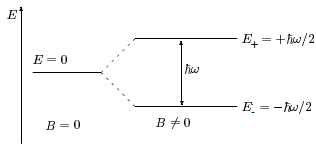
\includegraphics[scale=.9]{graphics/EieSpin.png}
\caption{Séparation du niveau fondamental en deux sous-niveaux en présence du
champ magnétique $\bls{B}$.}
\label{fig:EieSpin}
\end{wrapfigure}
L'hamiltonien qui décrit dans l'espace des états l'évolution du quanton dans
le champ $\bls{B}$ est
\begin{equation}
H=-\gamma BS_z=\omega S_z.
\end{equation}
Il est clair que $[H,S_z]=0$, donc les états propres de $S_z$ sont
des états stationnaires%
\begin{equation}
H\ket{+}=\frac{\hbar\omega}{2}\ket{+},~H\ket{-}=-\frac{\hbar\omega}{2}\ket{-}.
\end{equation}
Le champ magnétique $\bls{B}$ provoque donc l'apparition de deux niveaux
d'énergie séparés par $\hbar\omega$ comme on peut le voir sur la figure
\ref{fig:EieSpin}.

\subsubsection{Rotation et état de spin d'orientation arbitraire}
\label{sec:SpinArbitr1}

\begin{figure}[ptbh]
\begin{minipage}[c]{.45\linewidth}
\centering
  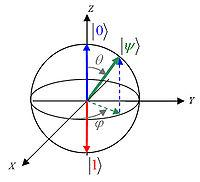
\includegraphics[scale=1]{graphics/SphereBloch.jpg}
\caption{Représentation 3D d'un spin $\frac{1}{2}$ sur une sphère de Bloch:
$\ket{\psi} =e^{-i\varphi/2}\cos\frac{\theta}{2}\ket{+}
+e^{i\varphi/2}\sin\frac{\theta}{2}\ket{-}$, avec $\ket{+}\equiv\ket{0}$,
$\ket{-}\equiv\ket{1}$.}
\label{fig:ReprSpin12Bloch}
\end{minipage} \hfill
\begin{minipage}[c]{.48\linewidth}
\centering
\ifcase\msipdfoutput
  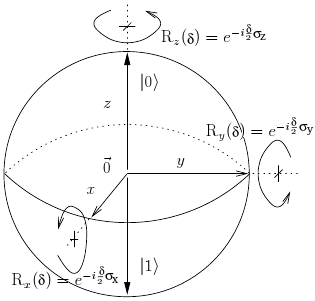
\includegraphics[scale=.7]{graphics/SphereBloch2.png}
\else
  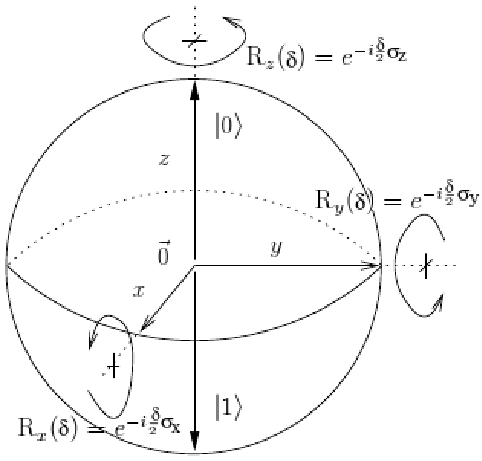
\includegraphics[scale=.7]{graphics/SphereBloch2.pdf}
\fi
\caption{Opérateurs rotations d'un single-qubit.}%
\label{fig:SphereBloch2}%
\end{minipage}

\end{figure}

Afin de fabriquer un qubit dans état de spin d'orientation arbitraire (comme
$\ket{\psi}$ sur la figure \ref{fig:ReprSpin12Bloch}) faisons tourner la
direction du champ magnétique du filtre de Stern et Gerlach et alignons le dans
la direction arbitraire
\begin{equation}
\bls{\hat{u}}(\theta,\varphi)=(\sin\theta\cos\varphi,
\sin\theta\sin\varphi,\cos\theta).
\end{equation}

Ainsi, seule la composante $B_{\bls{u}}=\bls{B}\cdot\bls{\hat{u}}$ du champ
magnétique est non nulle. Avec cette nouvelle orientation, le filtre de Stern et
Gerlach va fabriquer des états $\ket{\pm_{u}}$, obtenus en sélectionnant les
atomes déviés respectivement dans les sens $\pm \bls{\hat{u}}$. Ces états sont
vecteurs propres de l'opérateur%
\begin{equation}
\begin{split}
\sigma_{\bls{u}} & =\bls{\vec{\sigma}}\cdot\bls{\hat{u}}
=\sigma_{x}\sin\theta\cos\varphi+\sigma_{y}\sin\theta\sin\varphi+\sigma_z
\cos\theta\\
& =\begin{pmatrix}
\cos\theta & e^{-i\varphi}\sin\theta\\
e^{i\varphi}\sin\theta & -\cos\theta
\end{pmatrix}.
\end{split}
\end{equation}
Autrement,
\begin{equation}
\ket{+}_{u}=\binom{e^{-i\varphi/2}\cos\frac{\theta}{2}}{e^{i\varphi/2}\sin\frac{
\theta}{2}},\,\ket{-}_{u}=\binom{-e^{-i\varphi/2}\sin\frac{\theta}{2}}{e^{
i\varphi/2}\cos\frac{\theta}{2}}.
\end{equation}

Les états $\ket{+}_{u}$ et $\ket{-}_{u}$ sont les transformés des états par une
rotation qui amène l'axe $Oz$ sur l'axe $\bls{\hat{u}}$. Un choix possible
consiste à faire une première rotation de $\theta$ autour de l'axe $Oy$, suivie
d'une rotation de $\varphi$ autour de l'axe $Oz$.

En effet, sur la sphère de Bloch qu'illustre la figure \ref{fig:SphereBloch2},
les rotations d'angle $\delta$ autour des axes $Ox$, $Oy$ et $Oz$ sont générées,
en vertu de l'équation (\ref{eq:ExpoB}), par les opérateurs,%

\begin{subequations}
\begin{align}
R_{x}(\delta)  &
=e^{-i\frac{\delta}{2}\sigma_{x}}=\mathbb{I}\cos\frac{\delta}{2}
-i\sigma_{x}\sin\frac{\delta}{2}=\begin{pmatrix}
cos\frac{\delta}{2} & -i\sin\frac{\delta}{2}\\
-i\sin\frac{\delta}{2} & \cos\frac{\delta}{2}
\end{pmatrix},\\
R_{y}(\delta)  &
=e^{-i\frac{\delta}{2}\sigma_{y}}=\mathbb{I}\cos\frac{\delta}{2}
-i\sigma_{y}\sin\frac{\delta}{2}=\begin{pmatrix}
\cos\frac{\delta}{2} & -\sin\frac{\delta}{2}\\
\sin\frac{\delta}{2} & \cos\frac{\delta}{2}
\end{pmatrix},\\
R_z(\delta)  &
=e^{-i\frac{\delta}{2}\sigma_z}=\mathbb{I}\cos\frac{\delta}{2}
-i\sigma_z\sin\frac{\delta}{2}=\begin{pmatrix}
e^{-i\frac{\delta}{2}} & 0\\
0 & e^{+i\frac{\delta}{2}}
\end{pmatrix}.
\end{align}%
\end{subequations}%

Pour un axe de rotation quelconque de vecteur unitaire $\bls{\hat{u}}%
=(\bls{\hat{u}}_{x},\bls{\hat{u}}_{y},\bls{\hat{u}}_z)$,
on a%
\begin{equation}
R_{\bls{\hat{u}}}(\delta)=e^{-i\frac{\delta}{2}(\bls{\hat{u}}
\cdot\sigma
)}=\mathbb{I}\cos\frac{\delta}{2}-(\bls{\hat{u}}\cdot\sigma)i\sin\frac
{\delta}{2},
\end{equation}
où
$\bls{\hat{u}}\cdot\sigma=u_{x}\sigma_{x}+u_{y}\sigma_{y}+u_z\sigma_z
$.

Les matrices de Pauli étant hermitiennes, les opérateurs de rotation
$R_{\bls{\hat{u}}}(\delta)$ sont unitaires:
\begin{equation}
R_{\bls{\hat{u}}}^{\dagger}(\delta)=R_{\bls{\hat{u}}}(-\delta
)=R_{\bls{\hat{u}}}^{-1}(\delta).
\end{equation}

Dans la base standard $\{\ket{+},\ket{-}\}$, la matrice générale de rotation du
spin $\frac{1}{2}$ d'une rotation de $\theta$ autour de l'axe $Oy$ suivie d'une
rotation de $\varphi$ autour de l'axe $Oz$ est alors
\begin{equation}
\mathcal{D}^{1/2}(\theta,\varphi)=e^{-i\frac{\varphi}{2}\sigma_z}e^{-i\frac{
\theta}{2}\sigma_{y}}=\begin{pmatrix}
e^{-i\varphi/2}\cos\frac{\theta}{2} & -e^{-i\varphi/2}\sin\frac{\theta}{2}\\
e^{i\varphi/2}\sin\frac{\theta}{2} &
e^{i\varphi/2}\cos\frac{\theta}{2}
\end{pmatrix}.
\end{equation}

\medskip\colorbox[gray]{0.8}{
\parbox[c]{0.9\textwidth}{
\emph{Le fait le plus remarquable à propos dans l'expression de
$\mathcal{D}^{1/2}(\theta,\varphi)$ est qu'elle est multivoque: la
représentation d'une rotation de $\theta\ =2\pi$ est la matrice $-\mathbb{I}$,
alors que la rotation équivalente de $\theta\ =0$ ou $\theta\ =4\pi$ donne
$\mathbb{I}$. C'est une caractéristique des représentations de spin
demi-entier.}
}}
\medskip

L'ensemble des matrices $\mathcal{D}^{1/2}(\theta,\varphi)$ forme \textbf{le
groupe} $SU(2):$

\begin{itemize}
\item $S$: Spécial, i.e., $\det\mathcal{D}^{1/2}=+1$;

\item $U$: Unitaire, i.e.,
$(\mathcal{D}^{1/2})^{\dagger}=[\mathcal{D}^{1/2}]^{-1}$;

\item $2$: matrice $2\times2$.
\end{itemize}

\subsubsection{Évolution du qubit}

Supposons maintenant qu'à l'instant $t=0$, le quanton soit dans l'état propre
$\ket{+}_{u}$ de $S_{u}$,%
\begin{equation}
\ket{\psi(0)}=\ket{+}_{u}=e^{-i\varphi/2}\cos\frac{\theta}{2}\ket{+}
+e^{i\varphi/2}\sin\frac{\theta}{2}\ket{-}.
\end{equation}
qui n'est visiblement pas un état stationnaire. A un instant $t>0$, le quanton
est, d'après le \emph{postulat d'évolution}, dans l'état,
\begin{equation}%
\label{SpinT}%
\begin{split}
\ket{\psi(t)}&  =e^{-iHt/\hbar}\ket{\psi(0)}=e^{-i\omega t/2}e^{-i\varphi/2}\cos
\frac{\theta}{2}\ket{+}+e^{+i\omega t/2}e^{i\varphi/2}\sin\frac{\theta}{2}
\ket{-}\\
&  =e^{-i(\varphi+\omega t) /2}\cos\frac{\theta}{2}\ket{+} +e^{i(\varphi+\omega
t) /2}\sin\frac{\theta}{2}\ket{-}.
\end{split}
\end{equation}%
Il apparaît que si à $t=0$ le spin est orienté suivant la direction
$\bls{u}_0(\theta,\varphi)$, à l'instant $t$, il est orienté dans la
direction $\bls{u} _{t}(\theta,\varphi+\omega t)$. Au cours du temps, la
direction du spin tourne, dans le sens trigonométrique, autour de l'axe de
quantification $Oz$ à la vitesse angulaire $\omega=-\gamma B$, proportionnelle
au champ magnétique. Ce mouvement qui coïncide avec le mouvement du moment
magnétique classique porte le nom de \textbf{précession de Larmor}. On remarque
que c'est après $t_{etat}=\frac{4\pi}{\omega}$ que le quanton retrouve son état
initial.

D'après (\ref{SpinT}) lors d'une mesure de $\mathcal{S}_z$ à l'instant $t$
on obtient

\begin{enumerate}
\item $+\frac{\hbar}{2}$ avec une probabilité $|\langle +\ket{\psi(t)}|^{2}
=\cos^{2}\frac{\theta}{2}$;

\item $+\frac{\hbar}{2}$ avec une probabilité $|\langle -\ket{\psi(t)}|^{2}
=\sin^{2}\frac{\theta}{2}$.
\end{enumerate}

Ces probabilités sont bien évidemment indépendantes du temps puisque
$\ket{+}$ et $\ket{-}$ sont des états stationnaires.

La probabilité pour que, à l'instant $t$, le système retrouve son état de spin
initial $\ket{\psi(0)}\equiv\ket{+}_{u}$ est
\begin{equation}
\begin{split}
\mathcal{P}_{+}(t)&  =|_{u}\bra{+}\psi(t)\rangle|^{2}=|e^{-i\omega
t/2}\cos^{2}\frac{\theta}{2}+e^{+i\omega t/2}\sin^{2}\frac{\theta}{2}|^{2}\\
&  =\cos^{4}\frac{\theta}{2}+\sin^{4}\frac{\theta}{2}+\frac{1}{2}\cos^{2}%
\frac{\theta}{2}\sin^{2}\frac{\theta}{2}\cos\omega t.
\end{split}
\end{equation}
\emph{Les probabilités oscillent à une fréquence proportionnelle à la
fréquence de Larmor} $\omega=\frac{E_{+}-E_{-}}{\hbar}=\frac{\Delta E}{\hbar}$.
$\Delta E$ est la dispersion sur l'énergie: le quanton passe d'un niveau à
l'autre avec un temps caractéristique $\Delta t\simeq\frac{\hbar}{2\Delta E}$.

Si $\ket{+}_{u}\equiv\ket{+}_{x}$, alors $\theta=\frac{\pi}{2}$ et $\varphi=0$
et cette probabilité devient%
\begin{equation}
\mathcal{P}_{+}(t)=|_{x}\bra{+} \psi(t)\rangle|^{2}
=|\frac{1}{2}\left(e^{-i\omega t/2}+e^{+i\omega t/2}\right)|^{2}
=\cos^{2}\left( \frac{\omega t}{2}\right).
\end{equation}


Afin de comprendre cette précession du spin ou les oscillations des
probabilités, déterminons les valeurs moyennes des trois composantes du spin
$\frac{1}{2}$ dans l'état $\ket{\psi(t)}$:%
\begin{equation}
\bra{\psi(t)}S_z\ket{\psi(t)}=
\left(\frac{\hbar}{2}\right)\cos^{2}\frac{\theta}{2}+\left(-\frac{\hbar}{2}
\right)\sin^{2}\frac{\theta}{2}=\frac{\hbar}{2} \cos\theta.
\end{equation}
Cette valeur moyenne est sans surprise indépendante du temps puisque
$[H,S_z]=0$. En utilisant les expressions matricielles de $S_{x}$ et $S_{y}$,
on trouve sans difficulté
\begin{subequations}%
\label{MoySxSy}%
\begin{align}
\bra{\psi(t)} S_{x}\ket{\psi(t)} &
=\hbar\cos\frac{\theta}{2}\sin\frac{\theta}{2}\cos(\varphi+\omega t)
=\frac{\hbar}{2}\sin\theta\cos\left(\varphi+\omega t\right),\\
\bra{\psi(t)} S_{y}\ket{\psi(t)} &
=\hbar\cos\frac{\theta}{2}\sin\frac{\theta}{2}\sin(\varphi+\omega t)
=\frac{\hbar}{2}\sin\theta\sin\left(\varphi+\omega t\right).
\end{align}%
\end{subequations}%
$S_{x}$ et $S_{y}$ ne sont visiblement pas des constantes de mouvement. Les
équations (\ref{MoySxSy}) peuvent encore s'écrire%
\begin{equation}
\bra{\psi(t)} S_{x}+iS_{y}\ket{\psi(t)} =\frac{\hbar}{2}\sin\theta e^{i(\varphi
+\omega t)}=e^{i\omega t}(\bra{\psi(0)}S_{x}+iS_{y}\ket{\psi(0)}),
\end{equation}
montrant que $\langle \bls{S}(t)\rangle$ précesse autour de $Oz$ à la
fréquence $\omega$:%
\begin{equation}
\frac{d\left\langle \bls{S}\right\rangle }{dt}=\bls{\omega
}\wedge\left\langle \bls{S}\right\rangle.
\end{equation}
Après $t_{prec}=\frac{2\pi}{\omega},$ le quanton retrouve sa direction initiale.

A travers la valeur moyenne du spin, on retrouve le même comportement que le
moment magnétique classique.

Cette propriété, la précession, est à la base des techniques de
\textbf{résonance magnétique.}

\newpage


\section{Exercices et problèmes}

\subsection{Moment magnétique du deutéron}

Un noyau de deutérium plongé dans un champ magnétique $\bls{B}$ possède
trois états $\ket{+}$, $\ket{0} $, $\ket{-}$ d'énergie $+E_0$, $0$, $-E_0$
respectivement, avec $E_0=\hbar\omega$. Ce noyau a un moment magnétique et on
suppose que l'opérateur $M$ associé à la projection de ce moment sur une
direction fixe perpendiculaire au champ $\bls{B}$ a la forme
$M=\mu_0A,$ avec $\mu_0>0$ et $A$ défini par%
\begin{equation}
A\ket{+}=\frac{1}{\sqrt{2}}\ket{0},\,A\ket{0}=\frac{1}{\sqrt{2}}(\ket{+}+\ket{-}
),\,A\ket{-} =\frac{1}{\sqrt{2}}\ket{0} .
\end{equation}

\begin{enumerate}
\item Écrire la matrice représentant $A$ dans la base $\{\ket{+},\ket{0},\ket{-}
\}$. $A$ est-il hermitien?

\item Calculer les valeurs propres $m_1$, $m_2$ et $m_3$ de $M$ (avec
$m_1>m_2>m_3$) et déterminer les vecteurs propres normalisés correspondant 
$\ket{m_1}$, $\ket{m_2}$, $\ket{m_3}$.

\item On suppose qu'à l'instant $t=0$, le noyau est dans l'état
$\ket{\psi(0)}=\ket{m_1}$. Calculer $\ket{E}$ et $\Delta E$ dans cet état.

\item Calculer $\av{M}$ dans l'état $\ket{\psi(t)}$ en fonction de $\omega$.

\item Quelles sont, en fonction de $\omega$, les probabilités de trouver
$m_1$, $m_2$ et $m_3$ lors d'une mesure de $M$ sur l'état $\ket{\psi(t)}$?

\item Interpréter physiquement l'évolution de la composante transverse du
moment magnétique.
\end{enumerate}

\subsection{Précession de Larmor}

On considère un quanton de spin $\frac{1}{2}$ dont les états propres de
$S_z$ sont notés $\ket{+}_z$ et $\ket{-}_z$. On considère un état de spin
quelconque $\ket{\psi}$ caractérisé par les amplitudes de transition
$\alpha=_z\langle+\ket{\psi}$ et $\beta=_z\langle-\ket{\psi}$.

\begin{enumerate}
\item Quelle sont les probabilités des transitions $\ket{+}_z\longleftarrow
\ket{\psi}$ et $\ket{-}_z\longleftarrow\ket{\psi}$? Quelle relation doit lier
ces deux quantités?

\item On suppose que le quanton possède un moment magnétique $\bls{\mu
}$ et qu'il est placé dans un champ magnétique $\bls{B}=(0,0,B)$. Le
hamiltonien étant $H=-\bls{\mu}\cdot\bls{B}=\omega S_z$ avec
$\omega=-\gamma B$, quels sont les états stationnaires de ce quanton? Préciser
les énergies associées à ces états.

\item Si à l'instant $t=0$ le quanton est dans un état de spin qui soit état
propre d'une composante de $\bls{S}$ orthogonale à $\bls{B}$,
par exemple $S_{x}$. Notons $\ket{+}_{x}$ cet état.

\begin{enumerate}
\item Cet état est-il stationnaire?

\item Quelle est à l'instant $t>0$ et dans la base $\{\ket{+}_z,\ket{-}_z
\}$, l'amplitude de probabilité $_{x}\langle+\ket{\varphi(t)}$ si
$\varphi(0)=\ket{+}_{x}$?

\item Quelle est la probabilité $\mathcal{P}_{+}(t)=|_{x}\langle
+\ket{\varphi(t)}|^{2}$ pour que, à l'instant $t>0$, le quanton se retrouve dans
son état initial $\ket{+}_{x}$? Même question pour $\mathcal{P}_{-}(t)=
|_{x}\langle -\ket{\varphi(t)}|^{2}$.
\end{enumerate}

\item Les variations temporelles de ces probabilités sont le plus souvent
interprétées par référence à l'évolution des valeurs moyennes des composantes
du spin. Calculer ces valeurs moyennes dans l'état $\ket{\varphi(t)}$ et
conclure.

\item Le quanton est un neutron de longueur d'onde
$\lambda=1.55\opn{\mathring{A}}$ et masse $mc^{2}=939.566\opn{MeV}$.
On rappelle que $\hbar c=1\,973\opn{eV\mathring{A}}$.

\begin{enumerate}
\item Calculer la vitesse du neutron.

\item Déduire de la figure (\ref{fig:PrecLarmor}) la valeur de la vitesse
angulaire de précession du spin.

\item Le champ magnétique vaut $B=15.5\times10^{-4}\opn{T}$. En déduire
la valeur du moment magnétique du neutron.
\end{enumerate}
\end{enumerate}

\begin{figure}[ptbh]
\centering
\ifcase\msipdfoutput
	\includegraphics{graphics/PrecLarmor.eps}
\else
	\includegraphics{graphics/PrecLarmor.pdf}
\fi
\caption{Précession de Larmor des neutrons. Variation de $\langle
S_{x}\rangle _{\ket{\psi(t)}}$ en fonction de la
distance (c'est-à-dire du temps de parcours).}%
\label{fig:PrecLarmor}%
\end{figure}

\subsection{Détection des électrons}

Des électrons polarisés, avec des spins $\frac{1}{2}$ polarisés ($+$) dans la
direction $Oz$ pénètrent dans une région où règne un champ magnétique statique
$\bls{B}=(B_0,0,0)$. Les électrons se déplacent dans la direction $Oy$.
Après un temps $T$, les électrons atteignent un appareil de Stern-Gerlach où le
gradient de champ est orienté suivant $Oz$.

\begin{enumerate}
\item Écrire, dans la base qui diagonalise la matrice de Pauli $\sigma_z$, la
matrice du hamiltonien d'interaction $H_0$ dans la région où règne le champ
$\bls{B}=(B_0,0,0)$. On posera $\omega _0=-\gamma B_0$.

\item \label{q:ExoSpinDetec2}Sur un détecteur $D$ placé après l'appareil de
Stern-Gerlach, on ne peut détecter que les électrons de spin ($-$) dans la
direction $Oz$. Trouver les valeurs de $B_0$ qui permettent à tous les
électrons d'atteindre le détecteur $D$.

\item Pour la valeur minimale de $B_0$, de la question \ref{q:ExoSpinDetec2}, 
quel est le pourcentage des électrons qui atteignent $D$ si le temps de parcours 
dans la région où règne $B_0$ est $\frac{T}{2}$ et non $T$?
\end{enumerate}


\subsection{Réalisation expérimentale d'une porte logique 1-qubit}

On rappelle que le spin de l'électron \emph{génère} un moment magnétique
$\bls{\mu}=\gamma\bls{S}$, où $\gamma=g\frac{q}{2m}$ est le \emph{rapport
gyromagnétique} et $g$ est le \emph{facteur de Landé}.

L'hamiltonien qui décrit dans l'espace des états l'évolution de l'électron dans
le champ $\bls{B}=(0,0,B_0)$ est $\mathtt{H}=-\bls{\mu}\cdot\bls{B}$. On posera
$\omega_0=\gamma B_0$, la pulsation de Larmor ou pulsation de résonance.

On rappelle que l'opérateur de rotation autour de $Ou$ est
\begin{equation}
\mathtt{R}_u(\theta)= e^{-i\theta\sigma_{u}/2} =(\cos\frac{\theta}{2})\mathbb{I}
-i(\sin\frac{\theta}{2})\sigma_{u}.
\end{equation}
\begin{enumerate}
\item Donner, dans la base qui diagonalise $\mathtt{S}_z$, l'expression de la
matrice de $\mathtt{H}$ en fonction de $\omega_0$. Quels sont les niveaux
d'énergie du système?

\item Le vecteur d'état du spin, $\ket{\psi(t)}$ se décompose dans la base des
états propres de $\mathtt{S}_z$ sous la forme
\begin{equation}
\ket{\psi(t)} =\alpha_0(t)\ket{0}+\alpha_1(t)\ket{1}.
\end{equation}

\begin{enumerate}
\item En résolvant matriciellement l'équation de Schrödinger,
$i\hbar\frac{d}{dt}\ket{\psi(t)} =\mathtt{H}(t)\ket{\psi(t)}$, donner les
expressions de $\alpha_{0,1}(t)$, en fonction de $\alpha_{0,1}(0)$ et
$\mathtt{R}_z(\theta)$. On précisera l'expression de $\theta$.

\item Combien de temps faut-il laisser agir le champ magnétique statique
$\bls{B}_0$ sur le spin de l'électron pour réaliser, à un facteur de phase
globale près sur $\alpha_{0,1}(t)$, une porte q-logique $\mathtt{Z}$,
$\ket{k}\Qcircuit @C=1em @R=.7em { & \gate{\mathtt{Z}} & \qw}(-1)^{k}\ket{k}$?
Pourquoi ce facteur de phase globale est-il non-significatif du point de vue de
la mesure?
\end{enumerate}

\item Afin de réaliser une porte q-logique $\mathtt{X}$, $\ket{k}\Qcircuit
@C=1em @R=.7em {& \gate{\mathtt{X}} & \qw}\ket{1-k}$, on ajoute au champ
statique $\bls{B}_0$ un champ $\bls{B}_1(t)$ situé dans le plan $xOy$ tournant
dans le sens trigonométrique avec la vitesse angulaire $\omega$,
\begin{equation}
\bls{B}_1(t)=B_1(\bls{e}_{x}\cos\omega t+\bls{e}_{y}\sin\omega t) .
\end{equation}
On posera $\omega_1=\gamma B_1$ la \emph{fréquence ou pulsation de Rabi} et
$\delta=\omega+\omega_0$ \emph{le désaccord à la résonance}.

\begin{enumerate}
\item Écrire la nouvelle matrice du hamiltonien $\mathtt{H}(t)$ du système dans
la base où $\mathtt{S}_z$ est diagonale, puis le système d'équations
différentielles auquel obéissent $\alpha_{0,1}(t)$.

\item Pour résoudre ce système, on se place dans le référentiel tournant avec le
champ en posant
\begin{equation}
\alpha_0(t)=\beta_0(t)e^{-i\omega t/2},\,\alpha_1(t)=\beta_1(t)e^{+i\omega
t/2},\,\ket{\tilde{\psi}(t)}=\beta_0(t)\ket{0}+\beta_1(t)\ket{1}.
\end{equation}

\begin{enumerate}
\item Écrire $\ket{\tilde{\psi}(t)}$ en fonction de l'opérateur rotation
$\mathtt{R}_z$ et $\ket{\psi(t)}$ afin de justifier l'expression
\emph{référentiel tournant}.
\item Montrer que
\begin{equation}
i\hbar\begin{pmatrix}\dot{\beta}_0(t)\\\dot{\beta}_1(t)\end{pmatrix}
=\tilde{\mathtt{H}}\begin{pmatrix}\beta_0(t)\\\beta_1(t)\end{pmatrix},
\end{equation}
où $\tilde{\mathtt{H}}$ est fonction des matrices de Pauli et indépendant du
temps.

\item A partir de $\ket{\tilde{\psi}(t)}=\tilde{\mathtt{U}}(t)
\ket{\tilde{\psi}(0)}$, déduire la relation entre $\alpha_{0,1}(t)$ et
$\alpha_{0,1}(0)$ en fonction des matrices de Pauli.
\end{enumerate}
\end{enumerate}

\item Lorsque $\delta=0$, combien de temps faut-il laisser agir le champ
tournant pour réaliser, à un facteur de phase globale près, une porte qu-logique
$\mathtt{X}$?

\item A l'instant $t=0$, le spin est dans l'état pur $\ket{0}$.

\begin{enumerate}
\item Quelle est la probabilité $\mathcal{P}_{1\leftarrow0}(t)$ de trouver au
temps $t$ le spin dans l'état $\ket{1}$?

\item À quel instant cette probabilité est-elle maximale? Montrer que la porte
q-logique $\mathtt{X}$ consiste à faire basculer le spin de l'état $\ket{0}$ à
$\ket{1}$ et vice-versa. Quel est l'équivalent \emph{classique} de cette
opération logique quantique?
\end{enumerate}
\end{enumerate}

\subsection{QuTiP - Evolution d'un état de spin 1/2}

Écrire un programme (script) en Python utilisant QuTiP pour répondre aux 
questions suivantes.

L'évolution d'un quanton de spin 1/2, de moment magnétique $\mathbf{\mu}$, dans un champ magnétique $\textbf{B}(0,0,B)$, peut être décrit par l'hamiltonien $H=-\mathbf{\mu}.\textbf{B}=\omega S_z$. Le quanton pénètre dans le champ magnétique dans l'état $\ket{+}_x$. On prendra : $\hbar\omega=0.5$.
\begin{enumerate}
\item Définir l'hamiltonien $H$, ainsi que ses états propres $\ket{+}_z$ et $\ket{-}_z$.
\item Exprimer les états $\ket{+}_x$ et $\ket{-}_x$ en fonction des états propres du hamiltonien $H$.
\item Définir les projecteurs $P_+$ et $P_-$ respectivement sur les états $\ket{+}_x$ et $\ket{-}_x$
\item Le quanton initialement dans l'état $\ket{+}_x$ pénètre dans le champ magnétique à $t=0$. Résoudre l'équation de schr\"odonger, pour $t\in[0,30]$. Calculer en même temps les valeurs moyennes de $P_+$, $P_-$, $H$ et $H^2$.

\textbf{Note} : la valeur moyenne $\bra{\psi(t)}P_+\ket{\psi(t)}=\bra{\psi(t)}+\rangle_x ._x\langle+\ket{\psi(t)}=\mathcal{P}_+(t)$, est la probabilité de trouver le quanton à l'instant $t$ dans l'état $\ket{+}_x$. De même pour $P_-$.
\item Représenter, pour $t\in[0,30]$, les probabilités de trouver le quanton dans l'état $\ket{+}_x$ et $\ket{-}_x$. Que remarque-t-on?
\item Calculer pour $t=30s$ la déviation standard de $\Delta H$.
\end{enumerate}
